%!TEX encoding = UTF-8 Unicode
%!TEX root = ../labs.tex

\Lab{\LabWeekONE}
%\externaldocument{compendium}
\begin{Goals}
%!TEX encoding = UTF-8 Unicode

\item Kunna kombinera principerna sekvens, alternativ, repetition, och abstraktion i skapandet av egna program om minst 20 rader kod.
\item Kunna förklara vad ett program gör i termer av sekvens, alternativ, repetition, och abstraktion.
\item Kunna tillämpa principerna sekvens, alternativ, repetition, och abstraktion i enkla algoritmer.
\item Kunna formatera egna program så att de blir lätta att läsa och förstå.
\item Kunna förklara vad en variabel är och kunna skriva deklarationer och göra tilldelningar.
\item Kunna genomföra upprepade varv i cykeln \emph{editera-exekvera-felsöka/förbättra} för att successivt bygga upp allt mer utvecklade program.

\end{Goals}

\begin{Preparations}
\item Repetera veckans föreläsningsmaterial.
\item \DoExercise{\ExeWeekONE}{01}%Gör övning {\tt \ExeWeekONE} i kapitel \ref{exe:W01}.
\item Läs om Kojo i appendix \ref{appendix:kojo}. Kojo är förinstallerat på LTH:s datorer; om du vill installera Kojo på din egen dator, följ instruktionerna i \ref{appendix:ide:kojo:install}.
\item Läs igenom hela laborationen nedan. Fundera på möjliga lösningar till de uppgifter som är markerade med en penna i marginalen.
% \item Ladda hem och studera översiktligt detta dokument (25 sidor, det räcker att du bläddrar igenom dokumentet och får en uppfattning om hur Kojo kan användas): \\ ''Introduction to Kojo'' \url{http://www.kogics.net/kojo-ebooks#intro}
\end{Preparations}

\subsection{Obligatoriska uppgifter}

Om det förekommer en penna i marginalen ska du anteckna något inför redovisningen.


%%%%%%%%%%%%%%NEDAN ÄR FLYTTAT TILL ÖVNING 1 FÖR ATT GÖRA TYDLIGARE KOPPLING MELLAN LABBAR OCH ÖVN
%\Task \textit{Sekvens}.
%
%\Subtask Starta Kojo. Om du inte redan har svenska menyer: välj svenska i språkmenyn och starta om Kojo.  Skriv in nedan program och tryck på den \emph{gröna} play-knappen.
%
%\begin{Code}
%sudda
%
%fram; höger
%fram; vänster
%färg(grön)
%fram
%\end{Code}
%\noindent
%%Genom att börja din Kojo-program med \code{sudda} så startar du exekveringen i samma utgångsläge: en tom canvas där paddan pekar uppåt, pennan är nere och pennans färg är röd.
%%Då blir det lättare att resonera om vad programmet gör från början till slut, jämfört med om exekveringen beror på resultatet av tidigare exekveringar.
%
%\Subtask\Pen Vad händer om du \emph{inte} börjar programmet med \code{sudda} och kör samma program upprepade gånger? Varför är det bra att börja programmet med \code{sudda}?
%
%\Subtask Rita en kvadrat enligt bilden nedan.
%\vspace{1em}\\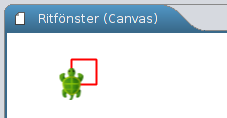
\includegraphics[width=0.45\textwidth]{../img/kojo/kvadrat}
%
%\Subtask Prova olika sätt att skriva din kod \emph{utan} att resultatet ändras: skriv satser i sekvens på flera rader eller satser i sekvens på samma rad med semikolon emellan; använd blanktecken och blanka rader i koden. Hur vill du gruppera dina satser så att de är lätta för en människa att läsa?
%
%\Subtask Prova att ändra på \emph{ordningen} mellan satserna och studera hur resultatet påverkas. Använd den \emph{gula} play-knappen  (programspårning) för att studera exekveringen i detalj. Klicka på satser i ditt program och på rutor i programspårningen och se vad som händer.
%
%
%\Subtask Rita en trappa enligt bilden nedan.
%
%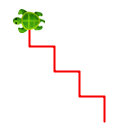
\includegraphics[width=0.2\textwidth]{../img/kojo/stairs}
%
%\Subtask Rita valfri bild på valfri bakgrund med hjälp av några av procedurerna i tabellen nedan. Du kan till exempel rita en rosa triangel med lila konturer mot svart bakgrund. % \ref{lab:kojo:kojo-procedures}.
%Försök att underlätta läsbarheten av din kod med hjälp av lämpliga radbrytningar och gruppering av satser. Undersök hur ordningen av satserna i din kod påverkar resultatet.
%
%
%
%\begin{table}[H]
%\begin{tabular}{l l}\small
%\code|fram(100)| & Paddan går framåt 100 steg (25 om argument saknas).\\
%\code|färg(rosa)| & Sätter pennans färg till rosa. \\
%\code|fyll(lila)| & Sätter ifyllnadsfärgen till lila. \\
%\code|fyll(genomskinlig)| & Gör så att paddan \emph{inte} fyller i något när den ritar. \\
%\code|bredd(20)| & Gör så att pennan får bredden 20. \\
%\code|bakgrund(svart)| & Bakgrundsfärgen blir svart. \\
%\code|bakgrund2(grön,gul)| & Bakgrund med övergång från grönt till gult. \\
%\code|pennaNer|  & Sätter ner paddans penna så att den ritar när den går. \\
%\code|pennaUpp|  & Sänker paddans penna så att den \emph{inte} ritar när den går. \\
%\code|höger(45)|   & Paddan vrider sig 45 grader åt höger. \\
%\code|vänster(45)| & Paddan vrider sig 45 grader åt vänster. \\
%\code|hoppa|       & Paddan hoppar 25 steg utan att rita. \\
%\code|hoppa(100)|  & Paddan hoppar 100 steg utan att rita. \\
%\code|hoppaTill(100, 200)| & Paddan hoppar till läget (100, 200) utan att rita. \\
%\code|gåTill(100, 200)|    & Paddan vrider sig och går till läget (100, 200). \\
%\code|öster|   & Paddan vrider sig så att nosen pekar åt höger. \\
%\code|väster|  & Paddan vrider sig så att nosen pekar åt vänster. \\
%\code|norr|    & Paddan vrider sig så att nosen pekar uppåt. \\
%\code|söder|   & Paddan vrider sig så att nosen pekar neråt. \\
%\code|mot(100,200)|   & Paddan vrider sig så att nosen pekar mot läget (100, 200) \\
%\code|sättVinkel(90)| & Paddan vrider nosen till vinkeln 90 grader. \\
%\end{tabular}
%%\label{lab:kojo:kojo-procedures}
%%\caption{Några användbara procedurer i Kojo.}
%\end{table}


%%% NEDAN ÄR BORTTAGEN FÖR ATT MINSKA MÄNGDEN ARBETE

%\Subtask \emph{Rita och mät}.
%\begin{itemize}[noitemsep]
%\item Börja ditt program med dessa satser:\\ \code{sudda; axesOn; gridOn; sakta(0); osynlig}
%\item Rita sedan en kvadrat som har 444 längdenheter i omkrets.
%\item Ta fram linjalen med höger-klick i ritfönstret och mät så exakt du kan hur lång diagonalen i kvadraten är. Skriv ner resultatet. \\ \emph{Tips:} Du kan zooma med mushjulet om du håller nere Ctrl-knappen. Du kan flytta linjalen om du klick-drar på linjalens skalstreck. Du kan vrida linjalen om du klickar på skalstrecken och håller nere Shift-tangenten.
%\item Kontrollera med hjälp av \code{math.hypot} och \code{println} vad det exakta svaret är. Skriv ner svaret med 3 decimalers noggrannhet. Du kan t.e.x. använda REPL i ett terminalfönster bredvid, eller öppna ett nytt extra Kojo-fönster i Arkiv-menyn, eller lägga in utskrifterna sist i ditt befintliga program. Utskrifter med \code{println} i Kojo sker i utdatafönstret.
%\end{itemize}
%
%\Subtask Rita en liksidig triangel med sidan 300 längdenheter genom att ge lämpliga argument till \code{fram} och \code{höger}. Vinklar anges i grader.
%
%\Subtask\Checkpoint Visa dina resultat för en handledare och diskutera hur uppgifterna ovan illustrerar principen om sekvens.

\vspace{1em}
\Task Starta Kojo (se övning {\tt \ExeWeekONE} i kapitel \ref{exe:W01}).


\Task \textit{Sekvens och repetition}.

\Subtask Rita en kvadrat med hjälp av proceduren \code+upprepa(n){ ??? }+ där du ersätter \code{n} med antalet repetitioner och \code{???} med de satser som ska repeteras.

\Subtask Kör ditt program med den \emph{gula} play-knappen för programspårning. Studera exekveringssekvensen. Klicka på anropen i programspårningsfönstret och studera markeringarna i ritfönstret.





\Task \textit{Variabel och repetition}

\Subtask Funktionen \code{System.currentTimeMillis} ingår i Javas standardbibliotek och ger ett heltal av typen \code{Long} med det nuvarande antalet millisekunder sedan midnatt den första januari 1970.  Med Kojo-proceduren \code{sakta(0)} blir det ingen fördröjning när paddan ritar och utritningen sker så snabbt som möjligt. Prova nedan program och förklara vad som händer.
\begin{Code}
sudda; sakta(0)
val n = 800 * 4
val t1 = System.currentTimeMillis
upprepa(n){ upprepa(4){ fram; höger } }
val t2 = System.currentTimeMillis
println(s"$n kvadratvarv tog ${t2 - t1} millisekunder")
\end{Code}

\Subtask\Pen Anteckna ungefär hur många kvadratvarv per sekund som paddan kan rita när den är som snabbast. Kör flera gånger eftersom den virtuella maskinen behöver ''värmas upp'' för att maskinkoden ska optimeras. Vissa körningar kan gå långsammare om skräpsamlaren behöver lägga tid på att frigöra minne.

\Subtask\Pen Vad har variablerna i koden ovan för namn? Vad har variablerna för värden?

\Subtask Rita en kvadrat igen, men nu med hjälp av en \code{while}-sats och en loopvariabel. Studera exekveringen med programspårning (den gula play-knappen).

\begin{Code}
sudda; sakta(100)
var i = 0
while (???) { fram; höger; i = ??? }
\end{Code}

\Subtask\Pen Vad är det för skillnad på variabler som deklareras med \code{val} respektive \code{var}?

\Subtask Rita en kvadrat igen, men nu med hjälp av en \code{for}-sats. Skriv ut värdet på den lokala variabeln \code{i} i varje loop-runda.

\begin{Code}
for (i <- 1 to ???) { ??? }
\end{Code}

\Subtask\Pen Går det att tilldela variabeln \code{i} ett nytt värde i loopen?

\Subtask\Pen Går det att referera till namnet \code{i} utanför loopen?


\Subtask Rita en kvadrat igen, men nu med hjälp av \code{foreach}. Skriv ut loopvariabelns värde i varje runda.

\begin{Code}
(1 to ???).foreach{ i => ??? }
\end{Code}

%\Subtask\Pen För var och en av de fyra repetitionskonstruktionerna du sett ovan, \code{upprepa}, \code{while}, \code{for} och \code{foreach}: skriv kod med penna på papper som skriver ut de första 100 jämna heltalen med blanktecken emellan: \code{2 4 6 8 10 12 ...} etc.\\ Vilken typ av loop tycker du är enklast att använda i detta fall?


\Task \textit{Abstraktion}.

\Subtask Använd en repetition för att abstrahera nedan sekvens, så att programmet blir kortare:
\begin{Code}
sudda

fram; höger; hoppa; fram; vänster; hoppa; fram; höger;
hoppa; fram; vänster; hoppa; fram; höger; hoppa; fram;
vänster; hoppa; fram; höger; hoppa; fram; vänster; hoppa;
fram; höger; hoppa; fram; vänster; hoppa
\end{Code}

%\Subtask\Pen Sök på nätet efter ''DRY principle programming'' och beskriv med egna ord vad DRY betyder och varför det är en viktig princip.

\Subtask Definiera en egen procedur som heter \code{kvadrat} med hjälp av nyckelordet \code{def} som vid anrop ritar en kvadrat med hjälp av en \code{for}-loop.

\begin{Code}
def kvadrat = for (???) {???}
\end{Code}


\Subtask Anropa din abstraktion efter att den deklarerats och efter att du exekverat:\\\code{sudda; sakta(100)}


\Subtask Anropa din abstraktion inuti en \code{for}-loop så att paddan ritar en stapel som är 10 kvadrater hög enligt bilden nedan.

\begin{figure}
  \begin{multicols}{2}

  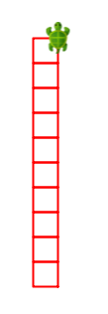
\includegraphics[scale=0.6]{../img/kojo/square-column}

  \columnbreak

  \begin{Code}
  def kvadrat = for (???) {???}
  for (???) {???}
  \end{Code}

  \end{multicols}
\end{figure}

\Subtask Kör ditt program med den \emph{gula} play-knappen. Studera hur anrop av proceduren \code{kvadrat} påverkar exekveringssekvensen av dina satser. Vid vilka punkter i programmet sker ett ''hopp'' i sekvensen i stället för att efterföljande sats exekveras? Använd lämpligt argument till \code{sakta} för att du ska hinna studera exekveringen.


\Subtask Rita samma bild med 10 staplade kvadrater som ovan, men nu \emph{utan} att använda abstraktionen \code{kvadrat} -- använd i stället en nästlad repetition (alltså en upprepning inuti en upprepning). Vilket av de två sätten (med och utan abstraktionen \code{kvadrat}) är lättast att läsa? %\emph{Tips:} Varje gång du trycker på någon av play-knapparna, sparas ditt program. Du kan se dina sparade program om du klickar på \emph{Historik}-fliken. Du kan också stega bakåt och framåt i historiken med de blå pilarna bredvid play-knapparna.

\Subtask Generalisera din abstraktion \code{kvadrat} genom att ge den en parameter \code{sida: Double} som anger hur stor kvadraten blir. Rita flera kvadrater i likhet med bilden nedan.

\begin{figure}[H]
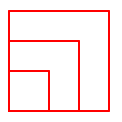
\includegraphics{../img/kojo/square-param}
\end{figure}



%\Subtask\Pen%\Checkpoint
%Se över ditt program i föregående uppgift och säkerställ att det är lättläst och följer en struktur som börjar med alla definitioner i logisk ordning och därefter fortsätter med huvudprogrammet.
%%Diskutera ditt program med en handledare.



%\Subtask\Pen Spara ditt program i en fil men lämpligt namn och ha programmet redo när det är din tur att redovisa vad du gjort under laborationen.
%Anteckna några åtgärder du vidtagit för att göra programmet mer lättläst.







\Task \emph{Alternativ.} \label{kojo:alt}

\Subtask Kör programmet nedan. Förklara vad som händer. Använd den gula play-knappen för att studera exekveringen.

\begin{Code}
sudda; sakta(5000)

def move(key: Int): Unit = {
  println("key: " + key)
  if (key == 87) fram(10)
  else if (key == 83) fram(-10)
}

move(87); move('W'); move('W')
move(83); move('S'); move('S'); move('S')
\end{Code}

\Subtask \label{subtask:keypress}  Kör programmet nedan. Notera \code{activateCanvas} för att du ska slippa klicka i ritfönstret innan du kan styra paddan. Anropet \code{onKeyPress(move)} gör så att \code{move} kommer att anropas då en tangent trycks ned. Lägg till kod i \code{move} som gör att tangenten A ger en vridning moturs med 5 grader medan tangenten D ger en vridning medurs 5 grader. Med \code{onKeyPress} bestämmer man vilken procedur som ska köras vid tangenttryck.

\begin{Code}
sudda; sakta(0); activateCanvas

def move(key: Int): Unit = {
  println("key: " + key)
  if (key == 'W') fram(10)
  else if (key == 'S') fram(-10)
}

onKeyPress(move)
\end{Code}



%\Subtask Spara ditt program i en fil men lämpligt namn och ha programmet redo när det är din tur att redovisa vad du gjort under laborationen.


\subsection{Kontrollfrågor}\Checkpoint

\noindent Repetera teorin för denna vecka och var beredd på att kunna svara på dessa frågor när det blir din tur att redovisa vad du gjort under laborationen:

\begin{enumerate}
\item Vad innebär sekventiell exekvering av satser?
\item Vad är skillnaden mellan en sats och ett uttryck?
\item Vad är skillnaden mellan en procedur och en funktion?
\item Spelar ordningen mellan argument någon roll vid anrop av en funktion med flera parametrar?
\item Vad är en variabel? Ge exempel på deklaration, initialisering och tilldelning av variabler, samt användning av variabler i uttryck.
\item Vad är en kontrollstruktur? Ge exempel på två olika slags kontrollstrukturer.
\item Vad är ett logiskt uttryck? Ge exempel på användning av logiska uttryck.
\item Vad är abstraktion? Ge exempel på användning av abstraktion.
\item Vad är nyttan med abstraktion?
\item Vad innebär sidoeffekt? Förklara och ge exempel.
\item Vad innebär tillstånd? Förklara och ge exempel.
\item Hur deklareras och initialiseras en variabel vars värde är förändringsbart?
\item Hur deklareras och initialiseras en variabel vars värde är oföränderligt?
\item Är det ett körtidsfel eller kompileringsfel att tilldela en oföränderlig variabel ett nytt värde?
\item Ange vilken av \code{for} och \code{while} är lämpligast i dessa fall:
\begin{itemize}[noitemsep, nolistsep]
\item[A.] Summera de hundra första heltalen.
\item[B.] Räkna antal tecken i en sträng innan första blanktecken.
\item[C.] Dra 100 slumptal mellan 1 och 6 och summera de tal som är mindre än 3.
\item[D.] Summera de första heltalen från 1 och uppåt tills summan är minst 100.
\end{itemize}
\end{enumerate}


\subsection{Frivilliga extrauppgifter}

\noindent Gör i mån intresse och träningsbehov nedan uppgifter i valfri ordning.

\Task \emph{Abstraktion och generalisering}.

\Subtask Skapa en abstraktion \code{def stapel = ???} som använder din abstraktion \code{kvadrat}.

\Subtask Du ska nu \emph{generalisera} din procedur så att den inte bara kan rita exakt 10 kvadrater i en stapel. Ge proceduren \code{stapel} en parameter \code{n} som styr hur många kvadrater som ritas.
\begin{Code}
def kvadrat = ???
def stapel(n: Int) = ???

sudda; sakta(100)
stapel(42)
\end{Code}



\Subtask Rita nedan bild med hjälp av abstraktionen \code{stapel}. Det är totalt 100 kvadrater och varje kvadrat har sidan 25. \emph{Tips:} Med ett negativt argument till procedur \code{hoppa} kan du få sköldpaddan att hoppa baklänges utan att rita, t.ex. \code{hoppa(-10*25)}

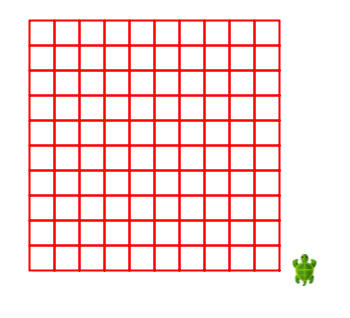
\includegraphics[width=0.3\textwidth]{../img/kojo/square-grid}

\Subtask Generalisera dina abstraktioner \code{kvadrat} och \code{stapel} så att man kan påverka storleken på kvadraterna som ritas ut.

\Subtask Skapa en abstraktion \code{rutnät} med lämpliga parametrar som gör att man kan rita rutnät med olika stora kvadrater och olika många kvadrater i både x- och y-led.

\Subtask Generalisera dina abstraktioner \code{kvadrat} och \code{stapel} så att man kan påverka fyllfärgen och pennfärgen för kvadraterna som ritas ut.

\Task \emph{Växling med booleska värden.}

\Subtask Bygg vidare på programmet i uppgift \ref{kojo:alt} och lägg till nedan kod i början av programmet. Lägg även till kod som gör så att om man trycker på tangenten G så sätts rutnätet omväxlande på och av. Observera att det är exakt \emph{en} procedur som anropas vid \code{onKeyPress}.

\begin{Code}
var isGridOn = false

def toggleGrid =
  if (isGridOn) {
    gridOff
    isGridOn = false
  } else {
    gridOn
    isGridOn = true
  }
\end{Code}

\Subtask Gör så att när man trycker på tangenten X så sätter man omväxlande på och av koordinataxlarna. Använd en variabel \code{isAxesOn} och definiera en abstraktion \code{toggleAxes} som anropar \code{axesOn} och \code{axesOff} på liknande sätt som i föregående uppgift.


\Task \emph{Repetition.}~Skriv en procedur \code{randomWalk} med detta huvud: \\
\code{def randomWalk(n: Int, maxStep: Int, maxAngle: Int): Unit}\\ som gör så att paddan tar \code{n} steg av slumpmässig längd mellan \code{0} och \code{maxStep}, samt efter varje steg vrider sig åt vänster en slumpmässig vinkel mellan \code{0} och \code{maxAngle}. Anropa din procedur med olika argument och undersök hur dess värden påverkar bildens utseende. \emph{Tips:} Uttrycket \code{math.random() * 100} ger ett tal från 0 till (nästan) 100. Du kan styra hur långsamt paddan ritar genom anrop av \code{sakta(???)} (prova dig fram till något  lämpligt heltalsargument i stället för \code{???}).
\vspace{2em}\\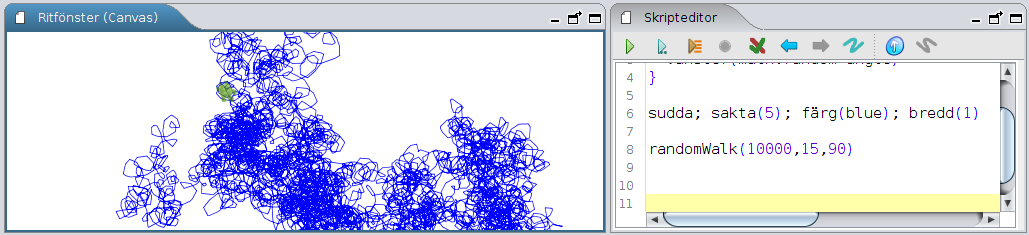
\includegraphics[width=\textwidth]{../img/kojo/random-walk.png}


\Task \emph{Variabler, namngivning och formatering.}

\Subtask Klistra in nedan konstigt formatterade program \emph{exakt} som det står med blanktecken, indragningar och radbrytningar. Kör programmet och förklara vad som händer.

\begin{figure}[H]
\begin{Code}
// Ett konstigt formaterat program med en del konstiga namn.

def gurka(x: Double,
y: Double, namn: String,
typ: String,
värde:String) = {
val tomat = 15
val h = 30
hoppaTill(x,y)
norr
skriv(namn+": "+typ)
hoppaTill(x+tomat*(namn.size+typ.size),y)
skriv(värde); söder; fram(h); vänster
fram(tomat * värde.size); vänster
fram(h); vänster
fram(tomat * värde.size); vänster }
sudda; färg(svart); val s = 130
val h = 40
var x = 42; gurka(10, s-h*0, "x","Int", x.toString)
var y = x; gurka(10, s-h*1, "y","Int", y.toString)
x = x + 1; gurka(10, s-h*2, "x","Int", x.toString)
gurka(10, s-h*3, "y","Int", y.toString); osynlig
\end{Code}
\end{figure}

\Subtask\Pen Skriv ner namnet på alla variabler som förekommer i programmet.

\Subtask\Pen Vilka av dessa variabler är lokala?

\Subtask\Pen Vilka av dessa variabler kan förändras efter initialisering?

\Subtask\Pen Föreslå tre förändringar av programmet ovan (till exempel namnbyten) som gör att det blir lättare att läsa och förstå.

\Subtask Gör sök-ersätt av \code{gurka} till ett bättre namn. \emph{Tips:} undersök kontextmenyn i editorn i Kojo genom att högerklicka. Använd kortkommandot för Sök/Ersätt.

\Subtask Gör automatisk formatering av koden med hjälp av lämpligt kortkommando. Notera skillnaderna. Vilka autoformateringar gör programmet lättare att läsa? Vilka manuella formateringar tycker du bör göras för att öka läsbarheten? Ge funktionen \code{gurka} ett bättre namn.  Diskutera läsbarheten med en handledare.



\Task \label{task:measuretime} \emph{Tidmätning.} Hur snabb är din dator?

\Subtask \label{task:timer} Skriv in koden nedan i Kojos editor och kör upprepade gånger med den gröna play-knappen. Tar det lika lång tid varje gång? Varför?

\begin{Code}
object timer {
  def now: Long = System.currentTimeMillis
  var saved: Long = now
  def elapsedMillis: Long = now - saved
  def elapsedSeconds: Double = elapsedMillis / 1000.0
  def reset: Unit = { saved = now }
}

// HUVUDPROGRAM:
timer.reset
var i = 0L
while (i < 1e8.toLong) { i += 1 }
val t = timer.elapsedSeconds
println("Räknade till " + i + " på " + t + " sekunder.")
\end{Code}


\Subtask Ändra i loopen i uppgift \ref{task:timer}) så att den räknar till 4.4 miljarder. Hur lång tid tar det för din dator att räkna så långt?\footnote{Det går att göra ungefär en heltalsaddition per klockcykel per kärna. Den första elektroniska datorn \href{https://sv.wikipedia.org/wiki/ENIAC}{Eniac} hade en klockfrekvens motsvarande 5 kHz. Den dator på vilken denna övningsuppgift skapades hade en i7-4790K turboklockad upp till 4.4 GHz.
%\href{http://www.extremetech.com/computing/185512-overclocking-intels-core-i7-4790k-can-devils-canyon-fix-haswells-low-clock-speeds/2}{www.extremetech.com/computing/185512-overclocking-intels-core-i7-4790k-can-devils-canyon-fix-haswells-low-clock-speeds/2}
}

\Subtask  Om du kör på en Linux-maskin: Kör nedan Linux-kommando upprepade gånger i ett terminalfönster. Med hur många MHz kör din dators klocka för tillfället? Hur förhåller sig klockfrekvensen till antalet rundor i while-loopen i föregående uppgift? (Det kan hända att din dator kan variera centralprocessorns klockfrekvens. Prova både medan du kör tidmätningen i Kojo och då din dator ''vilar''. Vad är det för poäng med att en processor kan variera sin klockfrekvens?)
\begin{REPLnonum}
> lscpu | grep MHz
\end{REPLnonum}


\Subtask Ändra i koden i uppgift \ref{task:timer}) så att \code{while}-loopen bara kör 5 gånger. Kör programmet med den \emph{gula} play-knappen. Scrolla i programspårningen och förklara vad som händer. Klicka på \code{CALL}-rutorna och se vilken rad som markeras i ditt program.

\Subtask Lägg till koden nedan i ditt program och försök ta reda på ungefär hur långt din dator hinner räkna till på en sekund för \code{Long}- respektive \code{Int}-variabler. Använd den gröna play-knappen.
\begin{CodeSmall}
def timeLong(n: Long): Double = {
  timer.reset
  var i = 0L
  while (i < n) { i += 1 }
  timer.elapsedSeconds
}

def timeInt(n: Int): Double = {
  timer.reset
  var i = 0
  while (i < n) { i += 1 }
  timer.elapsedSeconds
}

def show(msg: String, sec: Double): Unit = {
  print(msg + ": ")
  println(sec + " seconds")
}

def report(n: Long): Unit = {
  show("Long " + n, timeLong(n))
  if (n <= Int.MaxValue) show("Int  " + n, timeInt(n.toInt))
}

// HUVUDPROGRAM, mätningar:

report(Int.MaxValue)
for (i <- 1 to 10) report(4.26e9.toLong)
\end{CodeSmall}

\Subtask Hur mycket snabbare går det att räkna med \code{Int}-variabler jämfört med \code{Long}-variabler? Diskutera gärna svaret med en handledare.

\Task Lek med färg i Kojo. Sök på internet efter dokumentationen för klassen \code{java.awt.Color} och studera vilka heltalsparametrar den sista konstruktorn i listan med konstruktorer tar för att skapa sRGB-färger. Om du högerklickar i editorn i Kojo och väljer ''Välj färg...'' får du fram färgväljaren och med den kan du välja fördefinierade färger eller blanda egna färger. När du har valt färg får du se vilka parametrar till \code{java.awt.Color} som skapar färgen. Testa detta i REPL:

\begin{REPL}
scala> val c = new java.awt.Color(124,10,78,100)
c: java.awt.Color = java.awt.Color[r=124,g=10,b=78]

scala> c.  // tryck på TAB
asInstanceOf    getColorComponents      getRGBComponents
brighter        getColorSpace           getRed
createContext   getComponents           getTransparency
darker          getGreen                isInstanceOf
getAlpha        getRGB                  toString
getBlue         getRGBColorComponents

scala> c.getAlpha
res3: Int = 100
\end{REPL}
Skriv ett program som ritar många figurer med olika färger, till exempel cirklar som nedan. Om du använder alfakanalen blir färgerna genomskinliga.

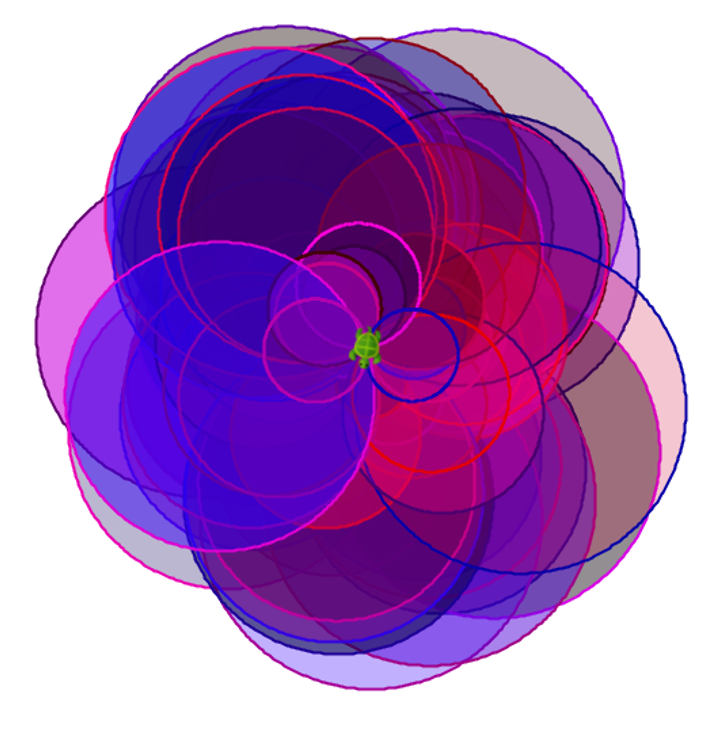
\includegraphics[width=0.82\textwidth]{../img/kojo/random-color-circles.png}


\Task Ladda ner ''Uppdrag med Kojo'' från \href{http://lth.se/programmera/uppdrag}{lth.se/programmera/uppdrag}  och gör några uppgifter som du tycker verkar intressanta.

%\Subtask ''Programming Fundamentals with Kojo'' som kan laddas ner här:\\
%\href{http://wiki.kogics.net/kojo-codeactive-books}{wiki.kogics.net/kojo-codeactive-books}

\Task Om du vill jobba med att hjälpa skolbarn att lära sig programmera med Kojo, kontakta \url{http://www.vattenhallen.lth.se} och anmäl ditt intresse att vara handledare.
